\section{Jackson und das Jackson-Projekt}\label{Jackson}
Das Jackson-Projekt entwickelt eine freie und modulare Bibliothek, f\"ur die Serialisierung und Deserialisierung von Java-Instanzen in \ac{JSON}-Dokumente und zur\"uck. Jackson wird unter der Contributor License Agreement (CLA) vermarktet. Die zur Zeit aktuelle Version ist 2.4.1, welche auch bei der Bearbeitung des Projektes eingesetzt wird.

\subsection{Jackson-Module}
Die Jackson-Bibliothek besteht aus verschiedenen Modulen, welche wie folgt bezeichnet und die folgenden Aufgabenbereiche haben:
\begin{itemize}
 \item "`jackson-core"', welches die JSON spezifische Implementierung sowie eine Low-Level-Streaming-API enth\"alt 
 \item "`jackson-databind"', welches f\"ur das \textit{Databinding} verantwortlich ist
 \item "`jackson-annotations"', welches die Jackson spezifischen Annotationen enth\"alt
 \item "`jackson-module-jaxb-annotations"' ist f\"ur die Verarbeitung von JAXB-Annotationen verantwortlich
 \item "`jackson-module-jsonSchema"', welches ein JSON-Schema f\"ur eine Klasse erstellt
\end{itemize}

Der Core enth\"alt die Low-Level-Streaming-API, welche die Kommunikation zwischen den einzelnen Modulen \"ubernimmt. Des Weiteren enth\"alt dieses Modul viele Grundklassen, die auch in anderen Modulen ben\"otigt werden.
Durch die grundlegenden Klassen und die Aufgabe als Kommunikationsvermittler wird das Modul \texttt{jackson-Core} immer ben�tigt, auch wenn dieses keine Aufgabe der Serialisierung im eigentlichen Sinn �bernimmt.

Unter "`Databind"' wird eine Methode verstanden, welche \"uber ein Userinterface gesteuert werden kann.
Dieses Modul ist in der Lage, Daten aus einem Datenstrom wie zum Beispiel einem JSON-File zu lesen oder zu schreiben.

Das "`Databind-Modul"' enth�lt somit den f�r \ac{JSON} notwendigen Scanner und Parser, welche die Umwandlung von Java-Klasse-Objekten in \ac{JSON}-Objeke und zur�ck �bernehmen.

Die Jackson-Annotations enthalten Informationen, die f\"ur das Serialisieren beziehungsweise Deserialisieren verantwortlich sind. Sie sind mit den \texttt{AnnotationInspectoren} in diesem Modul zusammengefasst.
Jackson kann aber auch Annotations von anderen Serialisierern erkennen und darauf reagieren.
Hierf�r wird ein weiteres Jackson-Modul ben\"otigt, welches in der Lage ist, die JAXB-Annotations zu verarbeiten (\texttt{jackson-module-jaxb-annotations}).

Annotations sind unter Jackson nicht zwingend f�r eine grundlegende Arbeitsweise des Serialisierers notwendig. Die Annotations werden jedoch f�r erweiterte Aufgaben wie zum Beispiel das Einschr\"anken des Wertebereichs eines Attributs ben�tigt.

Mit den drei Hauptmodulen \texttt{jackson-core}, \texttt{jackson-databind} und \texttt{jackson-annotations} ist die  Jackson-Bibliothek voll einsetzbar und kann Java-Instanzen zu einem JSON-Datenstrom umwandeln. Der JSON-Datenstrom wiederum kann gespeichert oder an andere Programme gesendet werden.

Um jedoch einheitliche Annotations f\"ur Jackson und JAXB zu haben, kommt das eben schon einmal angesprochene Modul \texttt{jackson-module-jaxb-annotations} zum Einsatz. Mit dessen Hilfe, Jackson in der Lage ist auch Annotations von JAXB zu verarbeiten.

Eine Mischung von Annotations verschiedener Serialisierer ist grunds\"atzlich m\"oglich, aber nicht empfehlenswert, da hier die \"Ubersichtlichkeit und die Verst\"andlichkeit des Codes leidet.
Aus diesem Grund wird hierauf in der Arbeit nicht weiter eingegangen.

Auch die Erstellung eines \ac{JSON}-Schemas aus einer Java-Klasse ist mit Hilfe des Moduls \texttt{jackson-module-jsonSchema} m\"oglich. Mit Hilfe von den Annotations kann dieses Schema erweitert werden. Die Erweiterungen beziehen sich haupts�chlich auf Werteberiche oder ver�nderte Namensgebung. Mit Annotations, welche f�r die Namensgebung verantwortlich sind, ist es m�glich, im \ac{JSON}-Dokument andere Namen zu verwenden als die Attributnamen.
Wie eine Schemaerzeugung genau funktioniert, wird im Kapitel \ref{JSON-Schema} genauer erkl\"art. \cite{Jackson}

\subsection{Serialisierung mit Jackson}\label{Serialisierung}
Der im folgenden beschriebene Sachverhalt erl\"autert das Quellcode-Listing auf der n�chsten Seite.

Um eine \textit{Minimal Exception Safety} zu garantieren wird nun eine \texttt{null}-Abfrage des zu serialisierenden Elements (\texttt{opmObject}) gemacht. Mit dieser Stufe der Sicherheit soll nicht verhindert werden, dass eine Exception passiert. Es wird lediglich garantiert, dass die Methode ohne abzust\"urzen durchlaufen werden kann. \cite{ExceptionSafety}

Um nun eine Serialisierung mit Jackson umzusetzen, wird zuerst eine Instanz der Klasse \\\texttt{ObjectMapper} ben\"otigt, welche den Databinder darstellt, welcher, wie schon dargestellt, den Datenstrom verarbeitet. Dieser \texttt{mapper} ist somit f\"ur die Konvertierung von Java-Instanzen zu JSON-Dokumenten verantwortlich. Das zu serialisierende Objekt ist im Beispiel \texttt{opmObject}, welches der Methode \texttt{serialize} \"ubergeben wird.

Jedoch wird nicht nur der \texttt{mapper} ben\"otigt, sondern auch ein \texttt{AnnotationInspector}, der jedoch abstrakt ist. Der \texttt{inspector} wird deshalb als Instanz von \texttt{JaxbAnnotationInspector} erstellt, was durch eine Implementierung der abstrakten Klasse m\"oglich ist. 
Weiterf�hrende �berlegungen zum \texttt{AnnotationInspector} sind im Kapitel \ref{SMDAnnotationInsector} n�her erl�utert.

Dem \texttt{inspector} wird eine \texttt{TypeFactory} mit "`Default-Einstellungen"' \"ubergeben . Dies bedeutet, es wird auf die Original JAXB-Annotations geparst, ohne auf Sonderf\"alle zu achten. Andere Annotations werden nicht ber\"ucksichtigt. Der \texttt{inspector} wird schlie\ss{}lich, nach der Erstellung, dem \texttt{mapper} \"ubergeben, damit dieser auf die entsprechnden Annotations reagieren kann.

Ist die zu serialisierende Instanz \texttt{null}, so wird eine \texttt{IllegalagumentException} generiert und die Methode so ordnungsgem\"a\ss{} beendet. Ist eine Instanz vorhanden, wird diese dem \texttt{mapper} \"ubergeben. Das Ergebnis des Aufrufs der Methode \texttt{writeValueAsString} von der Klasse \texttt{ObjectMapper} ist entweder bei Erfolg ein valider JSON-String oder beim Scheitern eine \\\texttt{JsonProcessingException}. 

Eine \texttt{JsonProcessingException} wird generiert, wenn Probleme beim parsen, beziehungsweise beim Generieren des \ac{JSON}-Kontent auftreten, die keine reinen I/O-Probleme sind. Die Exception erbt jedoch von \texttt{IOExecption}. Bei der \texttt{JsonProcessingException} handelt es sich um eine "`checked"' Exception welche irgendwo im Programmablauf abgefangen werden muss.

�ber den Methodenaufruf \texttt{writeValueAsString} wird also der Serialisierungsprozess mit der Jackson-Bibliothek in Gang gesetzt.

% Aus Gr�nden der Verst�ndlichkeit, wurde die \texttt{null}-Abfrage nicht am Methodenanfang gemacht, um bei einer Fehleingabe die Methode fr�hestm�glich zu verlassen, ohne vorher Objekte zu erstellen.
\newpage
\lstinputlisting{Code/Jackson_bsp.java}

\subsubsection{AnnotationInspector}\label{SMDAnnotationInsector}
Da wie eben schon einmal erkl�rt, der \texttt{AnnotationInspector} als abstrakte Klasse implementiert wurde, muss diese mit einer implementierten Instanz instanziiert werden. Dies kann wie im Kapitel \ref{Serialisierung} mit dem \texttt{JaxbAnnotationInspector} oder einem anderen \texttt{AnnotationInspector} geschehen.

Durch die Abstraktion der Klasse \texttt{AnnotationInspector} ist es m�glich, hier weitere Inspektoren zu implementieren. 

So w�re es zum Beispiel m�glich, einen \texttt{SMDAnnotationInspector} selber zu entwickeln, welcher nicht auf Annotations in einer Klasse achtet, sondern auf die im Projekt vorhandenen \ac{SMD} zur�ckgreift.

Mit dieser L�sung m�ssten keine Annotations an die eigentliche Klasse angebracht werden. Diese Informationen k�nnten durch den \texttt{SMDAnnotationInspector} direkt �ber den \ac{SMD}-Assistenten und der \ac{SMD}-Datenbank geladen werden. Eine genauere Beschreibung zum \ac{SMD}-Assistenten ist im Kapitel \ref{SMD-Assistent} zu finden.

% \newpage
\subsection{Deserialisierung mit Jackson}
Der im folgenden beschriebene Zusammenhang ist noch einmal im Quellcode-Listing auf der n�chsten Seite zu finden.

F\"ur die Deserialisierung mit Hilfe von Jackson wird wie bei der Serialisierung ebenfalls ein Databinder, also ein Objekt der Klasse \texttt{ObjectMapper} und ein \texttt{AnnotationInspector} ben\"otigt, welche wie im Kapitel \ref{Serialisierung} schon beschrieben, erstellt werden. 

Bevor dies jedoch passiert, wird gepr\"uft, ob der eingegebene String weder \texttt{null} noch \texttt{empty} ist, womit wieder die \textit{Minimal Exception Safety} garantiert werden kann. Sollte einer dieser F\"alle auftreten, so wird eine \texttt{IllegalArgumentException} zur\"uckgeliefert und die Methode ordnungsgem�� verlassen.

Wenn der String, wie eigentlich zu erwarten ist, einen Inhalt hat, wird die Methode \texttt{readValue} vom \texttt{mapper} mit dem \"ubergebenden String und der Information, um welche Klassen-Instanz es sich beim String handelt, \"ubergeben. Der zur\"uckgegebene Typ, der Methode \texttt{readValue}, entspricht dem Typ der im zweiten Argument \"ubergebenen Instanz.
Der Methodenaufruf \texttt{readValue} setzt somit unter Jackson die Deserialisierung in Gang.

Die Schwierigkeit beim Deserialisieren besteht nun darin, dass bevor der String \"uberhaupt deserialisiert werden kann, erst festgestellt werden muss, um welche Klasse es sich eigentlich handelt.

Im Codebeispiel unten wird momentan noch davon ausgegangen, dass es sich immer um eine Instanz der Klasse "`TestData"' handelt. Wie diese Einsch\"ankung aufgehoben werden kann, wird im folgenden Kapitel genauer beschrieben.

\lstinputlisting{Code/Jackson_des_bsp.java}

\subsection{Instanzunabh\"angige Deserialisierung}
Wie gerade schon erkl\"autert, wird beim Deserialisieren vorausgesetzt, dass der Typ der Instanz des zu deserialisierenden Strings bekannt ist.
Um den String nun eindeutig einem Typ zuzuordnen, musste eine eindeutige Kennzeichnung geschaffen werden.

Es wurde daraufhin in der Projektgruppe eine Einigung dar�ber getroffen, dass der Klassenname \"uber ein String-Attribut \texttt{className} hinzugef\"ugt wird. Aus diesem Grund bekam die Klasse \texttt{OPMObject} ein String-Attribut \texttt{className}, in welchem der Klassenname der jeweiligen Klasse abgelegt ist.

Durch die gemeinsame Wurzelklasse \texttt{OPMObject} haben nun alle Klassen das Attribut \texttt{className} geerbt. 
Daraus ergibt sich wiederum im Umkehrschluss, dass nur noch Klassen, welche von \texttt{OPMObject} erben, serialisiert werden k\"onnen, da nur sie mit Sicherheit das \texttt{className}-Attribut enthalten.
Beim Serialisieren wird nun der Klassenname mit in den Ausgabe-String geschrieben und dieser kann dadurch eindeutig identifiziert werden.

Um nun den Klassennamen aus dem String zu lesen, wurde die neue Methode \\\texttt{getClassFileFromString} geschrieben, welche den Klassennamen aus dem String filtert und diesen dann zur\"uckliefert. Das Auslesen des Typ-Namen wurde mit Hilfe der \texttt{split}-Methode der String-Klasse realisiert.

Diese Umsetzung ist vorl�ufig, da sie nicht effizient genug arbeitet, jedoch wesentlich schneller als Jacksons eigenes Parsen auf einen Schl\"usselnamen ist.\cite{Mkyong}

% \subsubsection{JSON-Parser}
�ber einen zus�tzlichen \ac{JSON}-Parser k�nnte der Effizenznachteil einer \texttt{split}-Methode, oder des Jackson-Parsers aufgehoben werden. Hierf�r gibt es unter Java verschiedene M�glichkeiten. So w�re eine Einbindung von \texttt{org.json}, \texttt{Gson}, \texttt{JSON.simple} oder \texttt{minimal-json} m�glich.\cite{EclipseSource}

Aus zeitlichen Gr\"unden, konnten keine Untersuchungen zu weiteren \ac{JSON}-Parsern gemacht werden. Jedoch wurde im Zuge der instanzunabh�ngigen Deserialisierung der Jackson-Parser getestet und f\"ur untauglich befunden, da er mindestens die zehnfache Zeit der \texttt{split}-Methode ben\"otigt.

% schau noch mal genau nach was es da von jackson gibt..............

\subsection{Klassendiagramm der Serialisierung}

Wie von OPM verlangt, erben hier alle Klassen von \texttt{OPMObject}. Um die Geschwindigkeit, beziehungsweise die Funktionalit\"at der XML- und JSON-Serialisierung vergleichen zu k\"onnen, wurde eine gemeinsame abstrakte Klasse \texttt{Serializer} erstellt. 

Die Klasse \texttt{JSONSerializer} erbt, um einen direkten Vergleich durchf\"uhren zu k\"onnen, genau wie \texttt{XMLSerializer} von \texttt{Serializer}.
\texttt{Testdata} und \texttt{TestData2OPM} sind erste Test-Klassen von denen Instanzen serialisiert und deserialisiert werden. Diese werden im sp\"ateren Verlauf des Projektes durch sinnvolle Testklassen ersetzt und sind sp\"ater nicht mehr aufzufinden.

Main-Klasse in diesem Projekt ist \texttt{OPM\_Serializer}. Die \texttt{main}-Methode setzt die Serialisierung zum Testen in Gang. Hierbei werden die Testklassen und die Serialisierer deklariert und instanziiert, welche f\"ur die Tests ben\"otigt werden.

Damit, wie gew\"unscht, jede Klasse serialisiert werden kann, wurde die Methode \texttt{serializeMe} zu \texttt{OPMObject} hinzugef\"ugt. Der Methode muss eine Instanz des Serialisierers \"ubergeben werden, welcher f\"ur die Serialisierung genutzt werden soll.

Durch die Vererbung im OPM-Modell, erbt jede Klasse die Methode \texttt{serializeMe}.
Diese Methode nutzt nun bei Aufruf die \texttt{serialize}-Methode des jeweiligen Serialisierers, um die Serialisierung durchzuf\"uhren.

Einen vollst�ndigen �berblick gibt das unten gezeigte Klassediagramm.


\begin{figure}[ht]
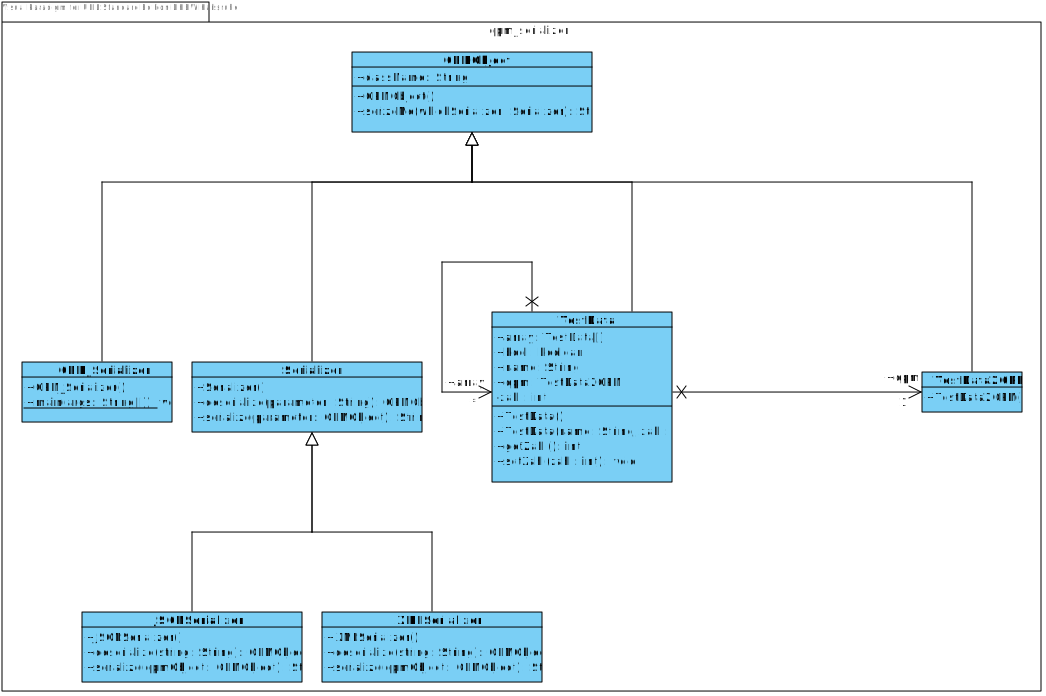
\includegraphics[width=16cm]{Bilder/Erstes_EKD}
\label{Klassendiagramm der Serialisierung}
\caption{Klassendiagramm der Serialisierung} 
\end{figure}
\FloatBarrier
\subsection{JSON-Schema-Erstellung aus einer Klasse}\label{JSON-Schema}
\"Ahnlich wie bei XML gibt auch es in JSON ein Datenformat, welches die zu erwartende Form des Streams vorgibt, das \ac{JSON}-Schema.
Wie in einer XSD, wird das Schema in der eigenen Norm als konformes Dokument erstellt. \cite{JSON_Schema}

Ein Beispiel f\"ur ein JSON-Schema wird hier anhand des \ac{JSON}-Dokuments in Kapitel \ref{Der Aufbau von JSON} dargestellt.
Das \ac{JSON}-Schema besteht aus einem Objekt, welches die jeweiligen Namen und Werte der Attribute einer Instanz enth\"alt und ist beispielhaft am Ende des Kapitels zu finden.

Somit steht am Anfang eines JSON-Schemas immer der Bezeichner \texttt{type} mit dem entsprechenden Wert, n\"amlich \texttt{object}. Dies ist zwingend erforderlich, da jedes \ac{JSON}-Dokument auch eine \ac{JSON}-Objekt ist.
Unter dem Schl\"ussel \texttt{properties} sind, wiederum als inneres Objekt, die Attribute mit ihren m\"oglichen Auspr\"agungen aufgelistet. 

Es gibt nat\"urlich weitere Bezeichner (\"ahnlich wie \texttt{type}), die den Wertebereich des Attributs weiter eingrenzen. Sie werden jedoch erst angezeigt, wenn die entsprechenden Annotations im Quellcode angebracht sind. Auf weitere Bezeichner wird im folgenden jedoch nicht weiter eingegangen, da dieses Thema zu umfangreich ist, um es in dieser Arbeit weiter zu vertiefen.

% Im Beispiel wird einfach nur der Typ des Attributs bezeichnet, jedoch ist es auch m\"oglich weitere Einschr\"ankungen \"uber Annotationen zu machen, wie eben schon erw\"ahnt wurde.

Am Anfang einer Property steht der Name des Atrributs, (im Beispiel \\\texttt{"}\texttt{stringValue"}), wie dargestellt.
Gefolgt wird dieser Name von einem Objekt, welches die genauen Eigenschaften des Attributs beschreibt.

Um die XML-Annotationen von JAXB bei der Schemaerzeugung zu nutzen, muss wieder ein \texttt{AnnotationInspector} verwendet werden. In diesem Fall ist das der \texttt{JaxbAnnotationInspector}.

Die Einschr\"ankungen und Beschreibungen der Attribute werden dem Serializer mit Hilfe der Annotationen \"ubergeben, welche Java-Methodennamen enthalten. 
Das Setzen der Beschreibungen geschieht \"uber Java-Methoden, welche zur Laufzeit vom Serializer aufgerufen werden.

\lstinputlisting{Code/JSON_Schema.json}

\subsection{JSON-Schema mit Hilfe von Jackson erstellen}
Seit der Jackson Version 2.2 wurde das Modul zur Erstellung eines JSON-Schemas \\(\texttt{"`jackson-modul-jsonSchema"'}) aus dem Modul \texttt{"`jackson-databind"'} ausgegliedert und ein eigenes Modul mit erweitertem Funktionsumfang eingef\"uhrt. 

F\"ur die Erstellung eines JSON-Schemas wird somit das Zusatzmodul \\\texttt{"`jackson-module-jsonSchema"'} ben\"otigt. Um unn\"otige Fehlerquellen zu vermeiden, wurde auch dieses Modul in der Version 2.4.1 verwendet, auch wenn es zum Erstellungsdatum schon eine neuere Version gab. Somit sind alle Module von der selben Version und Fehler durch Versionsunterschiede sind ausgeschlossen.

Im Codebeispiel unten wird der nun folgende Zusammenhang noch einmal verdeutlicht.

Wie schon in fr\"uheren Beispielen gezeigt, wird zuerst wieder ein \texttt{ObjectMapper} erstellt. Hierbei kann eine \texttt{JsonMappingException} auftreten, welche entweder weitergereicht werden kann oder direkt behandelt wird. Da die Exception "`checked"' ist, muss sie auf jeden Fall irgendwo im Programm behandelt werden.

Des Weiteren wird f\"ur die Schemaerzeugung noch ein \texttt{SchemaFactoryWrapper} erstellt, welcher das Schema erstellt.
Der Schema-Wrapper kann unter Umst\"anden die \texttt{JsonProcessingException} werfen, welche im Kapitel \ref{Serialisierung} genauer erl\"autert wird.

Der Wrapper wird nun, \"uber den n\"achsten Methodenaufruf, auf den Mapper und somit auf die entsprechend zu mappende Instanz angesetzt. Dies geschieht \"uber die Methode \\\texttt{acceptJsonFormatVisitor}.

Mittels der Methode \texttt{finalSchema} wird das Schema der Java-Klasse als \texttt{JsonSchema} erstellt.

\"Uber den \texttt{return}-Wert wird das \texttt{JsonSchema} als String \"ubergeben.

\lstinputlisting{Code/generateSchema.java}

\subsection{Auff\"alligkeiten beim Testen}
Beim Serialisieren und Deserialisieren sollen die Attributwerte einer Klasse in \ac{JSON}-Dokumenten gespeichert, beziehungsweise \ac{JSON}-Objekte in Attributwerte gewandelt werden. Hief\"ur ben\"otigen alle Klassen einen Standard-Konstruktor, damit der Serializer diesen beim Erstellen einer Klasseninstanz aufrufen kann, um eine "`neue"' Instanz zu erstellen.

Neu bedeutet in diesem Kontext, dass die Instanz zwar schon einmal existierte, aber zur jetzigen Laufzeit erst erstellt werden muss.

Des Weiteren ben\"otigt der Serializer f\"ur alle nicht \texttt{public} Attribute Getter- und Settermethoden, um Zugriff auf diese Attribute zu erhalten. Denn der Serializer darf durch Java-Richtlinien nur auf \texttt{public} Attribute ohne Getter- und Settermethoden zugreifen. Jedoch sollen nach \ac{OPM} keine Attribute \texttt{public} sein.

Um eine Serialisierung von allen Klassen zu gew\"ahrleisten, muss das \ac{OPM}-Modell angepasst werden. Denn laut \ac{OPM} sind Getter- und Settermethoden nicht zwingend notwendig und nur optional. Da diese Methoden aber f\"ur die Serialisierung notwendig sind, wurde \ac{OPM} angepasst und nun sind Getter- und Settermethoden Vorraussetzung.

Da alle Klassen sich an die \ac{OPM}-Regeln halten, ist somit wieder gew\"ahrleistet, dass alle ankommenden Instanzen serialisiert oder deserialisiert werden k\"onnen.

In ersten Tests mit dem \texttt{JSONSerializer} wurde die Funktionsf\"ahigkeit bewiesen. 

Es war nicht m\"oglich Klassen-Objekte getrennt von der anderen Klasse \"uber den Serialisierer zu trennen. Jedoch kann eine Trennung der Objekte auch manuell nach der Serialisierung vorgenommen werden.

\subsubsection{Auff\"alligkeiten beim Erstellen des JSON-Schemas}
Nach einigen Tests, wurde festgestellt, dass Jackson f\"ur alle Zahlen immer \texttt{integer} im Schema angibt, obwohl JSON auch \texttt{double} oder \texttt{float} kennt. Dabei ist es egal, ob es sich in der Klasse um \texttt{float, double} oder  \texttt{integer} handelt. Warum dies im Schema nicht ordnungsgem\"a\ss{} \"ubernommen wird, konnte trotz Recherche nicht herausgefunden werden.